\documentclass[tikz,border=4pt]{standalone}
\usepackage[T1]{fontenc}
\usepackage[utf8]{inputenc}
\usepackage{amsmath,amssymb}
\usepackage{helvet}
\renewcommand{\familydefault}{\sfdefault}
\usepackage{pgfplots}
\pgfplotsset{compat=1.17}
\usetikzlibrary{arrows.meta,positioning,calc,fit,backgrounds,shapes.geometric}

\definecolor{cVis}{HTML}{1F77B4}
\definecolor{cTxt}{HTML}{D62728}
\definecolor{cProj}{HTML}{2CA02C}
\definecolor{cLLM}{HTML}{9467BD}
\definecolor{cConv}{HTML}{FF7F0E}
\definecolor{cAtt}{HTML}{17BECF}
\definecolor{cGray}{HTML}{7F7F7F}

\tikzset{
  blk/.style={draw, rounded corners=2pt, minimum height=8mm, align=center, font=\footnotesize, thick},
  tok/.style={draw, minimum size=3.2mm, inner sep=0pt},
  arr/.style={-{Stealth[length=2mm]}, thick},
}

\begin{document}
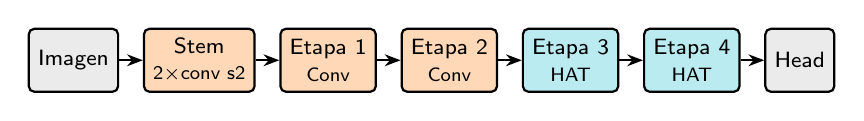
\begin{tikzpicture}[node distance=3mm]
  \node[blk, fill=black!8] (in) {Imagen};
  \node[blk, fill=cConv!30, right=of in] (st) {Stem\\\scriptsize 2$\times$conv s2};
  \node[blk, fill=cConv!30, right=of st] (s1) {Etapa 1\\\scriptsize Conv};
  \node[blk, fill=cConv!30, right=of s1] (s2) {Etapa 2\\\scriptsize Conv};
  \node[blk, fill=cAtt!30, right=of s2] (s3) {Etapa 3\\\scriptsize HAT};
  \node[blk, fill=cAtt!30, right=of s3] (s4) {Etapa 4\\\scriptsize HAT};
  \node[blk, fill=black!8, right=of s4] (hd) {Head};
  \foreach \a/\b in {in/st,st/s1,s1/s2,s2/s3,s3/s4,s4/hd}{\draw[arr] (\a) -- (\b);}
\end{tikzpicture}
\end{document}
